% Based on free LaTex template https://www.overleaf.com/latex/templates/modelo-tcc-computacao-atitus/dgwsczcmpczz
\documentclass[14pt]{article}

\usepackage{sbc-template}
\usepackage{graphicx, url}
\usepackage[utf8x]{inputenc}
\usepackage[T1]{fontenc}
\usepackage[english=american]{csquotes}
\usepackage{float}
\usepackage{comment}
\usepackage{amsmath}
\usepackage{amssymb}
\usepackage{enumerate}
\usepackage{subcaption}
\usepackage{setspace}
\usepackage{listings}
\usepackage{inconsolata}
\usepackage{tabularray}
\usepackage[english, russian]{babel}

%\usepackage[backref=page]{hyperref}
%\hypersetup{
%    colorlinks=true,
%    allcolors=blue,
%}

\usepackage[style=abnt]{biblatex}
\addbibresource{sbc-template.bib}

\usepackage{sty/cc_atitus}


\title{Раскрашивальщик}

\author{Бабанский Виталий, Бакин Денис}

\address{}


\begin{document}
\maketitle

\section{Постановка задачи}

Задача восстановления цветных изображений из черно-белых снимков является распространенной задачи и применяется, например,
при обновлении исторических снимков, которые были сделаны до изобретения цветной фотографии.
Более сложной постановкой той же задачи считается раскрашивание снимков NIR (near-infrared spectroscopy) ---
это снимки, где вместо количества видимого света фотосенсором камеры подсчитывается количестве фотонов с длиной волны
от 780 нм до 2500 нм, то есть выше видимого диапазона. Такая съемка применяется при низкой освещенности и
при съемке архитектурных объектов.

\begin{figure}[H]
    \centering
    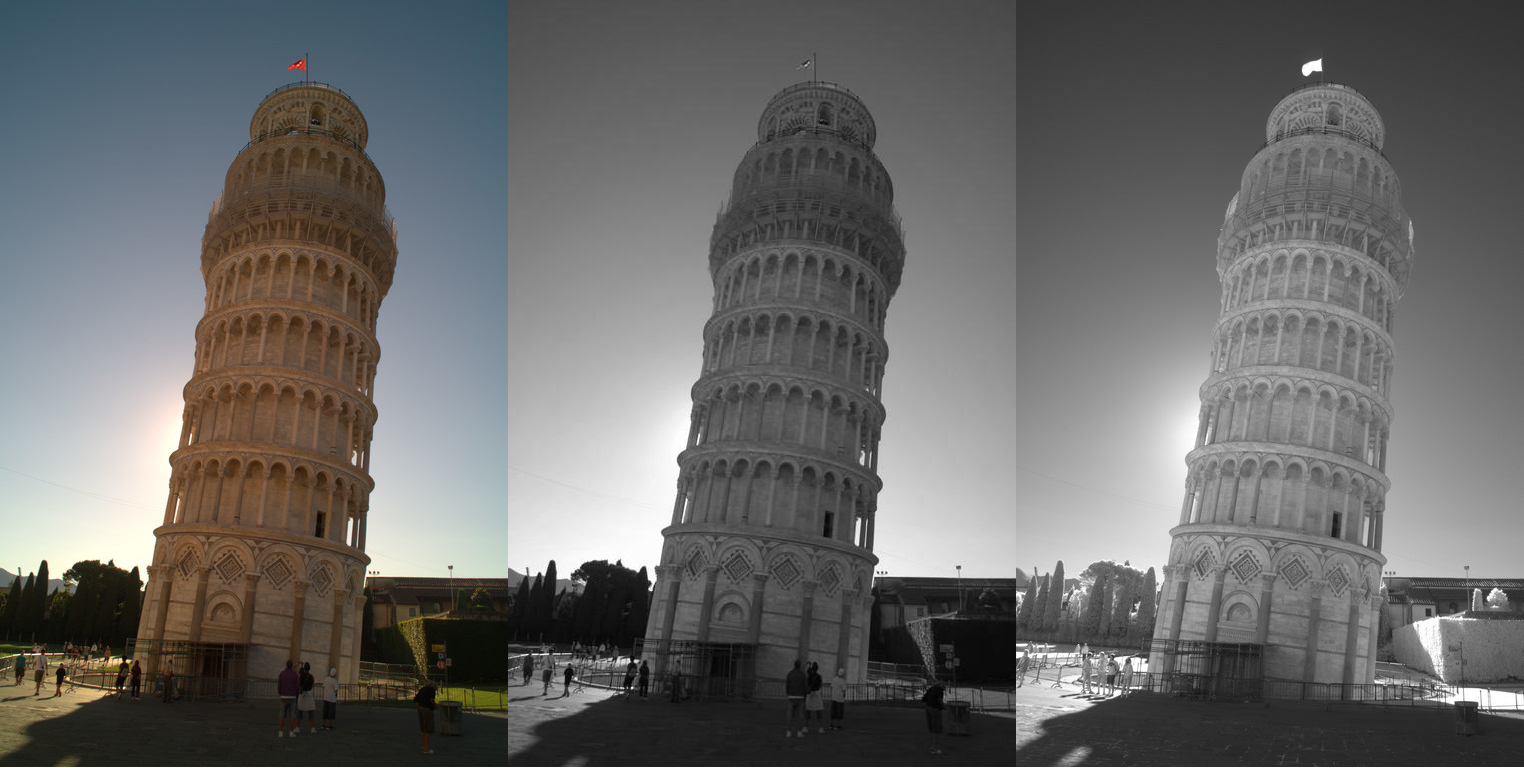
\includegraphics[width=0.5\textwidth]{resources/pisa_tower_3_colorspaces.jpg}
    \caption{Три пространства цветов: RGB, черно-белое и NIR}
    \label{fig:id_figura}
\end{figure}

\section{Постановка задачи}
Целью проекта является создание и обучение нейронной сети для получения цветных изображений по данным черно-белым изображениям.


\section{Литература}
Список рассмотренных не окончательный. Включены только те статьи, идеи которых скорее всего будут использовать в реализации.

В качества базовых моделей часто используется основная полносверточная нейронная сеть из \cite[numeric]{GuidedImageColorization}.

\section{Метрики качества}
Для оценки качества раскрашивания снимков будем использовать набор метрик. По ним же будем сравнивать качество работы моделей.

\begin{itemize}
    \item \textbf{MSE}. Один из наиболее очевидных методов оценки близости предсказания к "верному" ответу.
    К недостаткам этой метрики можно отнести неразличимость мелкой зашумленности и отсутствия контроля за резкими переходами цветов,
    которые требуются при корректном раскрашивании изображений.

    \item \textbf{PSNR (Пиковое отношение сигнал/шум)}: PSNR измеряет качество цветных изображений, сравнивая пиксельные различия между оригиналом и 
    раскрашенным изображением. Более высокие значения PSNR указывают на лучшее качество изображения с меньшими искажениями.

    \item \textbf{SSIM (Индекс структурного сходства)}: SSIM оценивает структурное сходство между оригиналом и раскрашенным изображением, 
    учитывая яркость, контрастность и текстуру. Этот индекс предоставляет более точную для восприятия меру качества изображения по сравнению 
    с метриками на основе пикселей, такими как PSNR.

    \item \textbf{AE (Абсолютная ошибка)}: AE количественно оценивает абсолютное различие между соответствующими пикселями оригинала и 
    раскрашенного изображения. Меньшие значения AE указывают на лучшую точность раскраски.

    \item \textbf{LPIPS (Обученное перцептуальное сходство изображений)}: LPIPS оценивает перцептуальное сходство с использованием моделей 
    глубокого обучения, фокусируясь на том, как человеческое зрение воспринимает различия между оригиналом и раскрашенным изображением. 
    Более низкие значения LPIPS означают, что раскрашенным изображение более точно соответствует восприятию человека.
\end{itemize}

\printbibliography

\end{document}
